\newif\ifsol
\soltrue
%==============================================================
%  EE201 -- Circuit Theory I
%  Example problems and solutions
%  M. Mert Ankaralı, METU EEE
%
%  Compile:  ./build.sh      (or: pdflatex EE201_Lecture_14.tex, twice)
%==============================================================
\documentclass[11pt,a4paper]{article}

%-------------------- packages --------------------------------
\usepackage[T1]{fontenc}
\usepackage[utf8]{inputenc}
\usepackage[english]{babel}
\usepackage{lmodern}
\usepackage[margin=2.3cm,top=2.0cm,bottom=1.9cm,headheight=14pt,headsep=9pt]{geometry}
\usepackage{amsmath,amssymb}
\usepackage{array,booktabs,tabularx}
\usepackage{enumitem}
\usepackage{needspace}
\usepackage[table]{xcolor}
\usepackage{fancyhdr}
\usepackage{titlesec}
\usepackage{graphicx}
\usepackage[most]{tcolorbox}
\usepackage{tikz}
\usepackage[american,siunitx]{circuitikz}
\usetikzlibrary{matrix,arrows.meta,positioning,calc,decorations.pathmorphing,decorations.pathreplacing,decorations.markings,patterns,shapes.geometric}
\usepackage[colorlinks=true,allcolors=metured,breaklinks=true]{hyperref}

%-------------------- colour system ---------------------------
% One colour per physical quantity, used identically in the slides.
\definecolor{metured}{RGB}{155,27,48}    % headings, structure
\definecolor{metugray}{RGB}{88,89,91}
\definecolor{ccur}{RGB}{0,102,170}       % CURRENT  -- blue
\definecolor{cvolt}{RGB}{214,120,0}      % VOLTAGE  -- orange
\definecolor{cpow}{RGB}{23,128,74}       % POWER / ENERGY -- green
\definecolor{ccharge}{RGB}{124,60,160}   % CHARGE   -- purple
\definecolor{cflux}{RGB}{0,138,138}      % FLUX -- teal
\definecolor{boxgray}{RGB}{245,245,245}
\definecolor{copper}{RGB}{184,98,30}

\newcommand{\Icol}[1]{\textcolor{ccur}{#1}}
\newcommand{\Vcol}[1]{\textcolor{cvolt}{#1}}
\newcommand{\Pcol}[1]{\textcolor{cpow}{#1}}
\newcommand{\Qcol}[1]{\textcolor{ccharge}{#1}}
\newcommand{\Fcol}[1]{\textcolor{cflux}{#1}}

%-------------------- units (no siunitx dependency) -----------
\newcommand{\uni}[1]{\,\mathrm{#1}}
\newcommand{\A}{\uni{A}}   \newcommand{\V}{\uni{V}}
\newcommand{\W}{\uni{W}}   \newcommand{\J}{\uni{J}}
\newcommand{\Cb}{\uni{C}}  \newcommand{\s}{\uni{s}}
\newcommand{\Sie}{\uni{S}} \newcommand{\Wb}{\uni{Wb}}

%-------------------- layout ----------------------------------
\pagestyle{fancy}
\fancyhf{}
\lhead{\small\textcolor{metugray}{EE201 -- Circuit Theory I}}
\rhead{\small\textcolor{metugray}{Example problems and solutions}}
\cfoot{\small\thepage}
\renewcommand{\headrulewidth}{0.4pt}

\titleformat{\section}{\large\bfseries\color{metured}}{\thesection.}{0.6em}{}
\titleformat{\subsection}{\normalsize\bfseries\color{metugray}}{\thesubsection.}{0.6em}{}
\titlespacing*{\section}{0pt}{1.4ex plus .3ex}{0.7ex}
\titlespacing*{\subsection}{0pt}{1.1ex plus .2ex}{0.5ex}

\setlist[itemize]{itemsep=2pt,topsep=3pt,parsep=0pt,leftmargin=1.5em}
\setlist[enumerate]{itemsep=2pt,topsep=3pt,parsep=0pt,leftmargin=1.7em}
\setlength{\parindent}{0pt}
\setlength{\parskip}{0.7ex plus .1ex}
\raggedbottom
\widowpenalty=10000
\clubpenalty=10000
\brokenpenalty=10000

%-------------------- boxes -----------------------------------
\newtcolorbox{definitionbox}[1]{enhanced,
  colback=metured!4, colframe=metured, boxrule=0.9pt,
  fonttitle=\bfseries, title={#1}, arc=2pt,
  left=7pt,right=7pt,top=5pt,bottom=5pt, before skip=7pt, after skip=7pt,
  before upper={\setlength{\parskip}{0.6ex plus .1ex}}}

\newtcolorbox{ideabox}[1][Key idea]{enhanced,
  colback=ccur!5, colframe=ccur, boxrule=0.9pt,
  fonttitle=\bfseries, title={#1}, arc=2pt,
  left=7pt,right=7pt,top=5pt,bottom=5pt, before skip=7pt, after skip=7pt,
  before upper={\setlength{\parskip}{0.6ex plus .1ex}}}

\newtcolorbox{examplebox}[1][Example]{enhanced,
  colback=cpow!4, colframe=cpow, boxrule=0.9pt,
  fonttitle=\bfseries, title={#1}, arc=2pt,
  left=7pt,right=7pt,top=5pt,bottom=5pt, before skip=7pt, after skip=7pt,
  before upper={\setlength{\parskip}{0.6ex plus .1ex}}}

%  Example solutions: a heading and numbered steps outside the example box
\newif\ifsolfirst
\newcommand{\solution}{\par\smallskip\noindent{\color{cpow}\bfseries Solution}\par\nobreak\smallskip\global\solfirsttrue}
\newcommand{\solstep}[2]{\par\ifsolfirst\global\solfirstfalse\else\medskip\needspace{5\baselineskip}\fi
  \noindent{\color{cpow}\bfseries Step #1.}\ {\bfseries #2}\par\nobreak\smallskip}

\newtcolorbox{cautionbox}[1][Careful]{enhanced,
  colback=cvolt!6, colframe=cvolt, boxrule=0.9pt,
  fonttitle=\bfseries, title={#1}, arc=2pt,
  left=7pt,right=7pt,top=5pt,bottom=5pt, before skip=7pt, after skip=7pt,
  before upper={\setlength{\parskip}{0.6ex plus .1ex}}}

%-------------------- circuitikz defaults ---------------------
%  voltage sources: smaller + and - inside the circle, further apart
\ctikzset{bipoles/vsourceam/inner plus={\tiny$+$},
          bipoles/vsourceam/inner minus={\tiny$\vphantom{+}-$},
          bipoles/vsourceam/margin=0.85,
          bipoles/cvsourceam/inner plus={\tiny$+$},
          bipoles/cvsourceam/inner minus={\tiny$\vphantom{+}-$},
          bipoles/cvsourceam/margin=0.85}
\ctikzset{bipoles/length=0.9cm, color=black,
          label/align=straight,
          bipoles/generic/height=0.28, bipoles/generic/width=0.62}
\tikzset{
  iar/.style={-{Stealth[length=2.2mm]}, ccur, thick},
  pol/.style={font=\small, text=cvolt},
  glab/.style={font=\footnotesize, text=metured},
  ttl/.style={font=\scriptsize\bfseries, text=metugray},
  capn/.style={font=\scriptsize, text=metugray, align=center},
  bigarr/.style={-{Stealth[length=3mm]}, very thick, metugray},
  gnode/.style={circle, fill=metured, inner sep=0pt, minimum size=4.4pt},
  nlab/.style={circle, draw=metured, text=metured, font=\scriptsize, inner sep=0.7pt},
  blab/.style={font=\footnotesize, text=black!80},
  gbr/.style={black!75, thick, postaction={decorate, decoration={markings,
      mark=at position 0.56 with {\arrow{Stealth[length=2.5mm]}}}}},
  apbr/.style={ccur, line width=1.7pt, postaction={decorate, decoration={markings,
      mark=at position 0.56 with {\arrow{Stealth[length=2.8mm]}}}}},
  hal/.style={draw=cpow!60, line width=6pt, opacity=0.35, line cap=round, line join=round},
  elem/.style={draw=metugray, thick, fill=metulight},
}
\definecolor{metulight}{RGB}{243,240,241}

%-------------------- Lecture 14 circuit macros ---------------
\newcommand{\ohm}{\,\Omega}
\newcommand{\yes}{\textcolor{cpow}{\checkmark}}
\newcommand{\e}[1]{\textcolor{cvolt}{e_{#1}}}
\newcommand{\nd}[1]{\tikz[baseline=(c.base)]\node[nlab](c){#1};}
\newcommand{\gnd}[2]{\draw (#1,#2) -- ++(0,-0.2) node[ground] {};}
\newcommand{\Rin}{R_{\mathrm{in}}}
%  Port variables in colour
\newcommand{\vone}{\Vcol{v_1}}  \newcommand{\vtwo}{\Vcol{v_2}}
\newcommand{\ione}{\Icol{i_1}}  \newcommand{\itwo}{\Icol{i_2}}
\newcommand{\Rm}{\mathbf{R}}  \newcommand{\Gm}{\mathbf{G}}
\newcommand{\Hm}{\mathbf{H}}  \newcommand{\Tm}{\mathbf{T}}
%  Labels beside a vertical element at (#1,#2), a fixed distance to the right (\lR) or left (\lL)
\newcommand{\lR}[3]{\node[anchor=west, xshift=7pt, font=\small] at (#1,#2) {#3};}
\newcommand{\lL}[3]{\node[anchor=east, xshift=-7pt, font=\small] at (#1,#2) {#3};}
\tikzset{tlab/.style={font=\small\bfseries, text=black!80},
         dotm/.style={circle, fill=black, inner sep=0pt, minimum size=4.2pt},
         core/.style={line width=1.1pt, metugray}}

%  Port 1 at terminals x = #1 (top y = #2, bottom y = 0): i_1 into the top terminal, + v_1 -
\newcommand{\pone}[2]{%
  \draw (#1,#2) node[ocirc] {}; \draw (#1,0) node[ocirc] {};
  \draw[iar] (#1+0.2,#2+0.28) -- (#1+0.75,#2+0.28); \node[font=\small, text=ccur] at (#1+0.48,#2+0.58) {$i_1$};
  \node[pol] at (#1+0.3,0.72*#2) {$+$}; \node[pol] at (#1+0.3,0.22*#2) {$-$};
  \node[font=\small, text=cvolt] at (#1+0.32,0.47*#2) {$v_1$};}
%  Port 2 at terminals x = #1: i_2 into the top terminal (pointing left), + v_2 -
\newcommand{\ptwo}[2]{%
  \draw (#1,#2) node[ocirc] {}; \draw (#1,0) node[ocirc] {};
  \draw[iar] (#1-0.2,#2+0.28) -- (#1-0.75,#2+0.28); \node[font=\small, text=ccur] at (#1-0.48,#2+0.58) {$i_2$};
  \node[pol] at (#1-0.3,0.72*#2) {$+$}; \node[pol] at (#1-0.3,0.22*#2) {$-$};
  \node[font=\small, text=cvolt] at (#1-0.32,0.47*#2) {$v_2$};}
%  A two-port box (text #1) with both ports
\newcommand{\tpbox}[1]{%
  \draw[elem] (1.0,-0.2) rectangle (3.4,2.2);
  \node[align=center, font=\small] at (2.2,1.0) {#1};
  \draw (0,1.8) -- (1.0,1.8); \draw (0,0) -- (1.0,0);
  \draw (3.4,1.8) -- (4.4,1.8); \draw (3.4,0) -- (4.4,0);
  \pone{0}{1.8} \ptwo{4.4}{1.8}}
%  A one-port box with a resistor-like port (for the review)
\newcommand{\opbox}[1]{%
  \draw[elem] (0,0) rectangle (1.9,2);
  \node[align=center, font=\small] at (0.95,1) {#1};
  \draw (1.9,1.7) -- (3.0,1.7) node[ocirc] {}; \draw (1.9,0.3) -- (3.0,0.3) node[ocirc] {};
  \draw[iar] (2.75,1.95) -- (2.2,1.95); \node[font=\small, text=ccur] at (2.48,2.25) {$i$};
  \node[pol] at (2.6,1.4) {$+$}; \node[pol] at (2.6,0.6) {$-$};
  \node[font=\small, text=cvolt] at (2.6,1.0) {$v$};}

%  Example 14.1: R_1 across port 1, R_2 across port 2 (no coupling)
\newcommand{\exTriv}{%
  \draw (0,1.8) -- (1.5,1.8); \draw (0,0) -- (1.5,0);
  \draw (1.5,1.8) to[R] (1.5,0); \lR{1.5}{0.9}{$2\ohm$}
  \draw (4.1,1.8) to[R] (4.1,0); \lL{4.1}{0.9}{$4\ohm$}
  \draw (4.1,1.8) -- (5.6,1.8); \draw (4.1,0) -- (5.6,0);
  \draw[dashed, metugray] (1.0,-0.45) rectangle (4.6,2.45);
  \pone{0}{1.8} \ptwo{5.6}{1.8}}

%  Example 14.2: R_1 (series), R_2 (shunt), CCVS 2 i_1 (+ on the left).
%  #1 = 0: both ports;  1: i_2 = 0 (port 2 open);  2: i_1 = 0 (port 1 open);  3: v_2 = 0 (port 2 shorted)
%  #2, #3: labels of R_1, R_2
\newcommand{\exTee}[4][2]{%
  \draw (0,2.2) -- (0.9,2.2) to[R, l=#3] (2.6,2.2) -- (4.3,2.2);
  \draw (4.3,2.2) to[american controlled voltage source, l=$\Vcol{#1\,i_1}$] (5.9,2.2) -- (6.9,2.2);
  \draw (2.6,2.2) to[R] (2.6,0); \lR{2.6}{1.1}{#4}
  \draw (0,0) -- (6.9,0);
  \fill (2.6,2.2) circle (1.7pt); \fill (2.6,0) circle (1.7pt);
  \ifcase#2
    \pone{0}{2.2} \ptwo{6.9}{2.2}
  \or
    \pone{0}{2.2}
    \draw (6.9,2.2) node[ocirc] {}; \draw (6.9,0) node[ocirc] {};
    \node[pol] at (6.6,1.6) {$+$}; \node[pol] at (6.6,0.5) {$-$};
    \node[font=\small, text=cvolt] at (6.58,1.05) {$v_2$};
    \node[font=\small, text=ccur, anchor=west] at (7.05,2.2) {$i_2 = 0$};
  \or
    \draw (0,2.2) node[ocirc] {}; \draw (0,0) node[ocirc] {};
    \node[pol] at (0.3,1.6) {$+$}; \node[pol] at (0.3,0.5) {$-$};
    \node[font=\small, text=cvolt] at (0.32,1.05) {$v_1$};
    \node[font=\small, text=ccur, anchor=east] at (-0.15,2.2) {$i_1 = 0$};
    \ptwo{6.9}{2.2}
  \or
    \pone{0}{2.2}
    \draw (6.9,2.2) -- (6.9,0);
    \draw[iar] (6.65,2.5) -- (6.1,2.5); \node[font=\small, text=ccur] at (6.38,2.8) {$i_2$};
    \node[font=\small, text=cvolt, anchor=west] at (7.05,1.1) {$v_2 = 0$};
  \fi}

%  Ideal transformer N_1 : N_2 as a two-port (coils at x = 1.4 and 3.0, height 1.8)
\newcommand{\xfmr}[2]{%
  \begin{scope}[xshift=#1 cm]
    \ctikzset{bipoles/length=1.2cm}
    \draw (0,0) to[L] (0,#2);
    \draw (1.6,#2) to[L] (1.6,0);
    \draw[core] (0.72,-0.05) -- (0.72,#2+0.05);
    \draw[core] (0.88,-0.05) -- (0.88,#2+0.05);
    \node[dotm] at (0.36,#2-0.2) {};
    \node[dotm] at (1.24,#2-0.2) {};
  \end{scope}}
\newcommand{\exXf}{%
  \draw (0,1.8) -- (1.4,1.8); \draw (0,0) -- (1.4,0);
  \xfmr{1.4}{1.8}
  \draw (3.0,1.8) -- (4.4,1.8); \draw (3.0,0) -- (4.4,0);
  \node[font=\small] at (2.2,2.2) {$N_1 : N_2$};
  \pone{0}{1.8} \ptwo{4.4}{1.8}}
\newcommand{\Rth}{R_{\mathrm{th}}}

%  Meters drawn upright: vertical (x, ytop, ybot, letter, label right) and horizontal (xl, xr, y, letter, label above)
\newcommand{\vmeter}[5]{%
  \draw (#1,#2) -- (#1,{(#2+#3)/2+0.32}); \draw (#1,{(#2+#3)/2-0.32}) -- (#1,#3);
  \node[circle, draw, thick, minimum size=0.64cm, inner sep=0pt, font=\small\bfseries] at (#1,{(#2+#3)/2}) {#4};
  \node[anchor=west, font=\small] at ({#1+0.38},{(#2+#3)/2}) {#5};}
\newcommand{\hmeter}[5]{%
  \draw (#1,#3) -- ({(#1+#2)/2-0.32},#3); \draw ({(#1+#2)/2+0.32},#3) -- (#2,#3);
  \node[circle, draw, thick, minimum size=0.64cm, inner sep=0pt, font=\small\bfseries] at ({(#1+#2)/2},#3) {#4};
  \node[anchor=south, font=\small] at ({(#1+#2)/2},{#3+0.36}) {#5};}
%  Test bench for a two-port in a box. #1 = 0: open-circuit test (current source at port 1,
%  voltmeters at both ports); 1: short-circuit test (voltage source at port 1, ammeters)
\newcommand{\bench}[1]{%
  \draw[thick, fill=gray!8] (3.0,-0.2) rectangle (5.0,2.4);
  \node[font=\large] at (4.0,1.1) {$N$};
  \draw (3.0,2.0) -- (2.6,2.0); \draw (3.0,0.2) -- (2.6,0.2);
  \draw (5.0,2.0) -- (5.4,2.0); \draw (5.0,0.2) -- (5.4,0.2);
  \foreach \p in {(2.6,2.0),(2.6,0.2),(5.4,2.0),(5.4,0.2)} \draw \p node[ocirc] {};
  \ifcase#1
    \draw (0,0.2) to[american current source, l=$\Icol{i_1}$] (0,2.0) -- (2.6,2.0);
    \draw (0,0.2) -- (2.6,0.2);
    \vmeter{1.5}{2.0}{0.2}{V}{$\Vcol{v_1}$}
    \fill (1.5,2.0) circle (1.6pt); \fill (1.5,0.2) circle (1.6pt);
    \draw (5.4,2.0) -- (6.6,2.0); \draw (5.4,0.2) -- (6.6,0.2);
    \vmeter{6.6}{2.0}{0.2}{V}{$\Vcol{v_2}$}
    \node[font=\small, text=ccur, anchor=south] at (6.0,2.05) {$i_2 = 0$};
  \or
    \draw (0,2.0) to[american voltage source, l_=$\Vcol{v_1}$] (0,0.2);
    \hmeter{0}{2.6}{2.0}{A}{$\Icol{i_1}$}
    \draw (0,0.2) -- (2.6,0.2);
    \draw (5.4,2.0) -- (6.6,2.0); \draw (5.4,0.2) -- (6.6,0.2);
    \vmeter{6.6}{2.0}{0.2}{A}{$\Icol{i_2}$}
    \node[font=\small, text=cvolt, anchor=south] at (6.0,2.05) {$v_2 = 0$};
  \fi}
%-------------------- recitation figures ----------------------
%  Question 1: a planar circuit (graph K_4) drawn with a crossing: R4 (1--3) and the 2 A source (2--4).
\newcommand{\nodeL}[3]{\node[nlab] at (#1,#2) {#3};}
\newcommand{\qOneNodes}{%
  \foreach \p in {(0,3.6),(6,3.6),(6,0),(0,0)} \fill \p circle (1.8pt);
  \nodeL{-0.4}{3.95}{1} \nodeL{6.4}{3.95}{2} \nodeL{6.4}{-0.35}{3} \nodeL{-0.4}{-0.35}{4}}
\newcommand{\qOneCommon}{%
  \draw (0,3.6) to[american voltage source, l_=$\Vcol{7\V}$] (0,0);        % + at node 1
  \draw (0,3.6) to[R, l=$R_1$] (6,3.6);
  \draw (6,3.6) to[R, l=$R_2$] (6,0);
  \draw (6,0) to[R, l=$R_3$] (0,0);
  \draw (0,3.6) -- (0.6,3.24) to[R, l_=$R_4$] (2.4,2.16) -- (6,0);}
\newcommand{\qOne}{%
  \qOneCommon
  \draw (6,3.6) -- (5.4,3.24) to[american current source, l_=$\Icol{2\A}$] (3.6,2.16) -- (3.214,1.929)
        arc[start angle=31, end angle=211, radius=0.25] -- (0,0);            % 2 A from node 2 to node 4
  \qOneNodes}
%  The same circuit without a crossing: the 2 A source goes around the outside; mesh currents
\newcommand{\mcw}[3]{% clockwise mesh current at (#1,#2), label #3
  \draw[-{Stealth[length=2mm]}, ccur, thick] (#1+0.42,#2) arc[start angle=0, end angle=-290, radius=0.42];
  \node[font=\small, text=ccur] at (#1,#2) {#3};}
\newcommand{\qOnePlanar}[1]{%
  \qOneCommon
  \draw (6,3.6) -- (8.4,3.6) to[american current source, l=$\Icol{2\A}$] (8.4,0) -- (8.4,-1.7)
        -- (-0.9,-1.7) -- (-0.9,0) -- (0,0);                                  % 2 A from node 2 to node 4
  \qOneNodes
  \ifnum#1=1 \mcw{4.5}{2.5}{$i_A$} \mcw{1.9}{0.95}{$i_B$} \mcw{7.4}{-0.85}{$i_C$}\fi}
%  Question 2: 24 V, 4 Ohm, 4 Ohm (v_x), 1 Ohm, VCCS v_x/4 from a to ground; port a--b
\newcommand{\qTwo}{%
  \draw (0,2.4) to[american voltage source, l_=$\Vcol{24\V}$] (0,0);        % + at the top
  \draw (0,2.4) to[R, l=$4\ohm$] (2.6,2.4) to[R, l=$1\ohm$] (5.0,2.4) -- (6.4,2.4);
  \draw (2.6,2.4) to[R, l=$4\ohm$] (2.6,0);
  \node[pol] at (2.15,1.75) {$+$}; \node[pol] at (2.15,0.65) {$-$};
  \node[font=\small, text=cvolt] at (2.1,1.2) {$v_x$};
  \draw (5.0,2.4) to[american controlled current source, l=$\Icol{v_x/4}$] (5.0,0);
  \draw (0,0) -- (6.4,0);
  \fill (2.6,2.4) circle (1.6pt); \fill (5.0,2.4) circle (1.6pt);
  \fill (2.6,0) circle (1.6pt); \fill (5.0,0) circle (1.6pt);
  \draw (6.4,2.4) node[ocirc] {}; \draw (6.4,0) node[ocirc] {};
  \node[font=\small, anchor=west] at (6.5,2.4) {a}; \node[font=\small, anchor=west] at (6.5,0) {b};}
%  Question 3: pi network 2 Ohm, 2 Ohm, 2 Ohm and a VCCS v_1/2 at port 2
\newcommand{\qThree}{%
  \draw (0,2.2) -- (1.3,2.2) to[R, l=$2\ohm$] (3.7,2.2) -- (7.6,2.2);
  \draw (1.3,2.2) to[R, l=$2\ohm$] (1.3,0);
  \draw (3.7,2.2) to[R, l=$2\ohm$] (3.7,0);
  \draw (5.2,2.2) to[american controlled current source, l=$\Icol{v_1/2}$] (5.2,0);
  \draw (0,0) -- (7.6,0);
  \foreach \x in {1.3,3.7,5.2} {\fill (\x,2.2) circle (1.6pt); \fill (\x,0) circle (1.6pt);}
  \pone{0}{2.2} \ptwo{7.6}{2.2}}
\tikzset{vax/.style={-{Stealth[length=2mm]}, gray!70}, crv/.style={very thick, line join=round}}

\begin{document}

%-------------------- title block -----------------------------
\begin{center}
\begin{tcolorbox}[enhanced, colback=metured!5, colframe=metured, boxrule=1pt,
                  arc=3pt, left=10pt,right=10pt,top=7pt,bottom=7pt, width=\textwidth]
\begin{center}
  {\small\scshape Middle East Technical University}\\[2pt]
  {\small\scshape Department of Electrical and Electronics Engineering}\\[7pt]
  {\Large\bfseries\color{metured} EE201 -- Circuit Theory I}\\[4pt]
  {\large\bfseries Example problems and solutions}\\[4pt]
  {\small Node and mesh analysis \quad$\cdot$\quad Th\'evenin and Norton equivalents \quad$\cdot$\quad two-port circuits}
\end{center}
\end{tcolorbox}
\end{center}



%==============================================================
\section*{Question 1 --- a planar circuit: node and mesh analysis}

\begin{center}
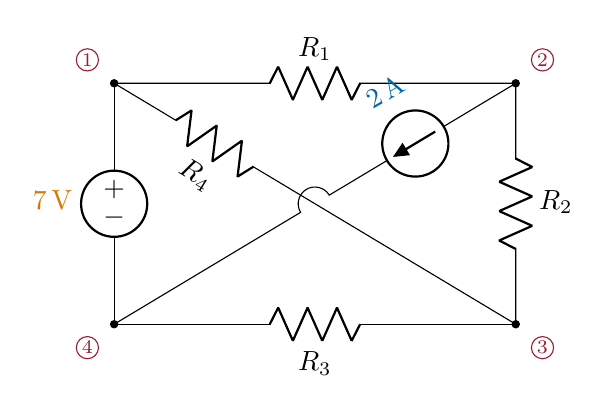
\begin{tikzpicture}[scale=0.85]
  \qOne
\end{tikzpicture}
\end{center}

$R_1 = R_2 = R_3 = 1\ohm$ and $R_4 = 2\ohm$. The resistor $R_4$ (nodes 1--3) and the $2\A$ source
(from node 2 to node 4) cross without a connection.
\begin{enumerate}[label=(\alph*)]
  \item The circuit is drawn with a crossing. Is it planar? If so, redraw it without a crossing.
  \item Node voltage analysis: take node 4 as the datum. How many unknown node voltages are
        there? Write KCL, then $Y_n\,\mathbf{e} = \mathbf{i}_n$, and solve.
  \item Mesh current analysis on your new drawing. How many unknown mesh currents are there?
        Write KVL, then the mesh equations in matrix form, and solve.
  \item Find the current of $R_4$ and the power delivered by the $7\V$ source with both
        results. Do they agree?
\end{enumerate}

\ifsol
\needspace{16\baselineskip}
\solution

\solstep{a}{Planar?}
There are $n = 4$ nodes and $b = 6$ branches, and every pair of nodes is joined by one branch.
The crossing is not needed: take the $2\A$ source around the outside. So the circuit is
\textbf{planar}, and mesh analysis applies. It has $b - n + 1 = 3$ meshes.
\begin{center}
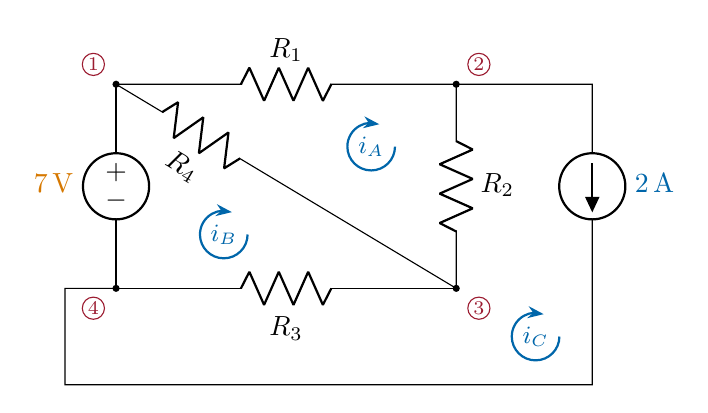
\begin{tikzpicture}[scale=0.72]
  \qOnePlanar{1}
\end{tikzpicture}
\end{center}
Mesh $A$: $R_1$, $R_2$, $R_4$. Mesh $B$: $R_4$, $R_3$ and the $7\V$ source. Mesh $C$: $R_2$, $R_3$
and the $2\A$ source. All mesh currents are clockwise.

\solstep{b}{Node voltage analysis}
\emph{Unknowns.} The datum is node 4, so $\Vcol{e_4} = 0$. The $7\V$ source is between node 1 and
the datum: $\Vcol{e_1} = 7\V$ is \textbf{known}. Unknowns: $\Vcol{e_2}$, $\Vcol{e_3}$.

\emph{KCL} (currents leaving the node):
\begin{align*}
  \text{node 2:}\quad & \frac{\Vcol{e_2} - 7}{1} + \frac{\Vcol{e_2} - \Vcol{e_3}}{1} + 2 = 0\\
  \text{node 3:}\quad & \frac{\Vcol{e_3} - \Vcol{e_2}}{1} + \frac{\Vcol{e_3}}{1}
                        + \frac{\Vcol{e_3} - 7}{2} = 0
\end{align*}
\emph{Matrix form.} Move the known terms to the right:
\[
  \underbrace{\begin{bmatrix} 2 & -1\\ -1 & 2.5 \end{bmatrix}}_{Y_n}
  \begin{bmatrix} \Vcol{e_2}\\ \Vcol{e_3} \end{bmatrix}
  = \underbrace{\begin{bmatrix} 7 - 2\\ 3.5 \end{bmatrix}}_{\mathbf{i}_n} \ \mathrm{(S,\ V,\ A)} .
\]
By inspection: a diagonal entry is the total conductance at the node ($1 + 1$; $1 + 1 + \frac12$),
an off-diagonal entry is minus the conductance between the two nodes. The right side holds the
source currents into the node, and $G\,\Vcol{e_1}$ for each conductance to the known node 1.

\emph{Solve.} Row 1 gives $\Vcol{e_3} = 2\,\Vcol{e_2} - 5$; row 2 then gives
$4\,\Vcol{e_2} - 12.5 = 3.5$:
\[
  \Vcol{e_2} = 4\V, \qquad \Vcol{e_3} = 3\V .
\]

\solstep{c}{Mesh current analysis}
\emph{Unknowns.} The $2\A$ source is only in mesh $C$, in its direction:
$\Icol{i_C} = 2\A$ is \textbf{known}. Unknowns: $\Icol{i_A}$, $\Icol{i_B}$.

\emph{KVL} (clockwise, voltage drops):
\begin{align*}
  \text{mesh } A:\quad & 1\cdot\Icol{i_A} + 1\,(\Icol{i_A} - \Icol{i_C})
                         + 2\,(\Icol{i_A} - \Icol{i_B}) = 0\\
  \text{mesh } B:\quad & 2\,(\Icol{i_B} - \Icol{i_A}) + 1\,(\Icol{i_B} - \Icol{i_C}) - 7 = 0
\end{align*}
Mesh $B$ goes up through the source, from $-$ to $+$: a rise of $7\V$. Mesh $C$ is not needed:
its KVL only adds the unknown voltage of the current source.

\emph{Matrix form.} Plug in $\Icol{i_C} = 2$ and move the known terms to the right:
\[
  \underbrace{\begin{bmatrix} 4 & -2\\ -2 & 3 \end{bmatrix}}_{Z_M}
  \begin{bmatrix} \Icol{i_A}\\ \Icol{i_B} \end{bmatrix}
  = \begin{bmatrix} 2\\ 7 + 2 \end{bmatrix} \ \mathrm{(\Omega,\ A,\ V)} .
\]
By inspection: a diagonal entry is the total resistance of the mesh ($1 + 1 + 2$; $2 + 1$), an
off-diagonal entry is minus the shared resistance ($R_4$).

\emph{Solve.} Row 1 gives $\Icol{i_A} = 0.5 + 0.5\,\Icol{i_B}$; row 2 then gives
$2\,\Icol{i_B} - 1 = 9$:
\[
  \Icol{i_A} = 3\A, \qquad \Icol{i_B} = 5\A .
\]

\solstep{d}{Compare}
\begin{center}
\small
\renewcommand{\arraystretch}{1.35}
\begin{tabular}{@{}lll@{}}
\toprule
 & \textbf{Node analysis} & \textbf{Mesh analysis}\\
\midrule
Unknowns & 2 ($\Vcol{e_1}$ fixed by the $7\V$ source) & 2 ($\Icol{i_C}$ fixed by the $2\A$ source)\\
$R_4$, from 1 to 3 & $(\Vcol{e_1} - \Vcol{e_3})/2 = (7 - 3)/2 = 2\A$ & $\Icol{i_B} - \Icol{i_A} = 5 - 3 = 2\A$\\
$7\V$ source, up & $\frac{7 - \Vcol{e_2}}{1} + \frac{7 - \Vcol{e_3}}{2} = 3 + 2 = 5\A$ & $\Icol{i_B} = 5\A$\\
\bottomrule
\end{tabular}
\end{center}
Both give the same answers. The source current is $5\A$, leaving its $+$ terminal: the source
\textbf{delivers} $7 \cdot 5 = 35\W$.

Quick check (optional): $R_1$, $R_2$, $R_3$ carry $3$, $1$, $3\A$ and $R_4$ carries $2\A$, so the
resistors absorb $9 + 1 + 9 + 2 \cdot 4 = 27\W$. The current source has $\Vcol{e_2} - \Vcol{e_4} = 4\V$
across it and absorbs $4 \cdot 2 = 8\W$: $27 + 8 = 35$. \ \yes
\fi
%==============================================================
\ifsol\needspace{14\baselineskip}\fi
\section*{Question 2 --- Th\'evenin, Norton and maximum power}

\begin{center}
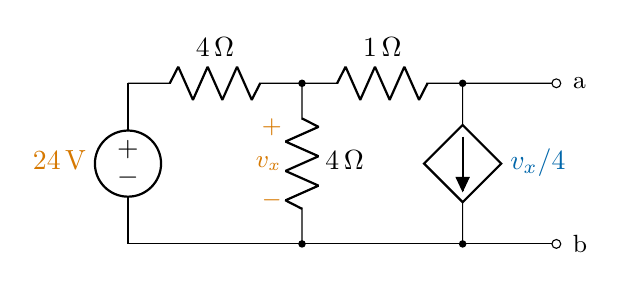
\begin{tikzpicture}[scale=0.85]
  \qTwo
\end{tikzpicture}
\end{center}

The dependent source is a voltage-controlled current source $v_x/4$ (in A, with $v_x$ in V).
\begin{enumerate}[label=(\alph*)]
  \item Find the Th\'evenin equivalent seen from the port a--b.
  \item Find the Norton equivalent.
  \item Check $R_{\mathrm{th}}$ with a test source. Why can it not be found by combining resistors?
  \item Which load resistor $R_L$ at a--b receives the maximum power? How much?
\end{enumerate}

\ifsol
\solution

\solstep{1}{Open circuit: $v_{\mathrm{oc}}$}
With a--b open, the $1\ohm$ resistor carries exactly the dependent source current $v_x/4$
(KCL at a). KCL at the top node of $v_x$:
\[
  \frac{24 - v_x}{4} = \frac{v_x}{4} + \frac{v_x}{4}
  \quad\Rightarrow\quad v_x = 8\V .
\]
Then $v_{\mathrm{oc}} = v_x - 1 \cdot \frac{v_x}{4} = 8 - 2 = 6\V$, so $v_{\mathrm{th}} = 6\V$.

\solstep{2}{Short circuit: $i_{\mathrm{sc}}$}
With a--b shorted, $v_a = 0$ and the $1\ohm$ resistor carries $v_x/1$. KCL at the top node:
\[
  \frac{24 - v_x}{4} = \frac{v_x}{4} + v_x
  \quad\Rightarrow\quad v_x = 4\V .
\]
KCL at a: $i_{\mathrm{sc}} = v_x - \frac{v_x}{4} = 3\A$. So $R_{\mathrm{th}} = v_{\mathrm{oc}}/i_{\mathrm{sc}} = 2\ohm$.
Th\'evenin: $6\V$ in series with $2\ohm$. Norton: $3\A$ in parallel with $2\ohm$.

\solstep{3}{Test source}
Kill the $24\V$ source (a short) but keep the dependent source. Apply $v$ at a--b. KCL at the
top node: $\frac{v_x}{4} + \frac{v_x}{4} + (v_x - v) = 0$, so $v_x = \frac23 v$. The test current
is
\[
  i = (v - v_x) + \frac{v_x}{4} = \frac{v}{3} + \frac{v}{6} = \frac{v}{2}
  \quad\Rightarrow\quad R_{\mathrm{th}} = \frac{v}{i} = 2\ohm . \ \yes
\]
Series--parallel combination ($4 \parallel 4 + 1 = 3\ohm$) gives the wrong answer: the dependent
source is not killed and changes the current.

\solstep{4}{Maximum power}
$R_L = R_{\mathrm{th}} = 2\ohm$, and
$P_{L,\max} = \dfrac{v_{\mathrm{th}}^2}{4 R_{\mathrm{th}}} = \dfrac{36}{8} = 4.5\W$.
\fi

%==============================================================
\ifsol\needspace{14\baselineskip}\fi
\section*{Question 3 --- a two-port with a dependent source}

\begin{center}
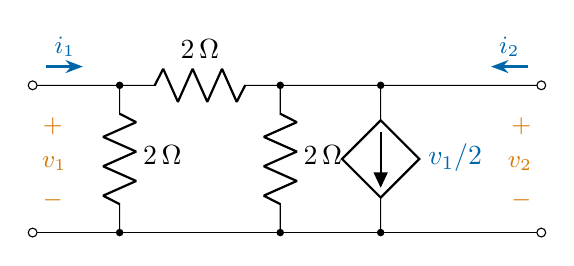
\begin{tikzpicture}[scale=0.85]
  \qThree
\end{tikzpicture}
\end{center}

The dependent source is a voltage-controlled current source $v_1/2$ (in A, with $v_1$ in V).
\begin{enumerate}[label=(\alph*)]
  \item Find the conductance matrix $\Gm$ by short-circuit tests.
  \item Find the resistance matrix $\Rm$. Check $r_{12}$ and $r_{22}$ with an open-circuit test.
  \item Find the hybrid matrix $\Hm$.
  \item Does the transmission matrix $\Tm$ exist? Explain.
  \item Is the two-port passive? (Write $P_N = \vone\,\ione + \vtwo\,\itwo$ in terms of $\vone$ and $\vtwo$.)
\end{enumerate}

\ifsol
\solution

\solstep{a}{$\Gm$ by short-circuit tests}
\emph{Port 2 shorted} ($\vtwo = 0$): the left and the middle $2\ohm$ are both across $\vone$, so
$\ione = \vone/2 + \vone/2 = \vone$. At the port-2 node, the middle resistor brings $\vone/2$
in and the dependent source takes $\vone/2$ out, so $\itwo = 0$:
$g_{11} = 1\Sie$, $g_{21} = 0$.

\emph{Port 1 shorted} ($\vone = 0$): the dependent source is $0$. Then
$\itwo = \vtwo/2 + \vtwo/2 = \vtwo$ and $\ione = -\vtwo/2$: $g_{22} = 1\Sie$, $g_{12} = -\frac12\Sie$.
\[
  \Gm = \begin{bmatrix} 1 & -\frac12\\[2pt] 0 & 1 \end{bmatrix} \mathrm{S} .
\]

\solstep{b}{$\Rm$}
$\det \Gm = 1$, so
\[
  \Rm = \Gm^{-1} = \begin{bmatrix} 1 & \frac12\\[2pt] 0 & 1 \end{bmatrix} \Omega .
\]
Check, port 1 open ($\ione = 0$): KCL at port 1 gives $\frac{\vone}{2} + \frac{\vone - \vtwo}{2} = 0$,
so $\vone = \vtwo/2$. KCL at port 2: $\itwo = \frac{\vtwo}{2} + \frac{\vtwo - \vone}{2} + \frac{\vone}{2} = \vtwo$.
So $r_{22} = \vtwo/\itwo = 1\ohm$ and $r_{12} = \vone/\itwo = \frac12\ohm$. \ \yes

\solstep{c}{$\Hm$}
The first row of $\Gm$ gives $\vone = \ione + \frac12\,\vtwo$; the second row gives $\itwo = \vtwo$:
\[
  \begin{bmatrix} \vone\\ \itwo \end{bmatrix}
  = \underbrace{\begin{bmatrix} 1\ohm & \frac12\\[2pt] 0 & 1\Sie \end{bmatrix}}_{\Hm}
    \begin{bmatrix} \ione\\ \vtwo \end{bmatrix} .
\]

\solstep{d}{$\Tm$}
$\Tm$ gives port 1 from port 2: $[\,\vone \ \ione\,]^T = \Tm\,[\,\vtwo \ {-\itwo}\,]^T$. Its
inputs are $\vtwo$ and $-\itwo$.

\emph{Test: set both inputs to zero.} Make port 2 dead: $\vtwo = 0$ and $\itwo = 0$. Row 2 of
$\Gm$ is $\itwo = \vtwo$, so this is allowed. Row 1 then gives $\ione = \vone$, and $\vone$ can
still be any value. A nonzero port 1 with a dead port 2: \textbf{$\Tm$ does not exist}.

\emph{Meaning.} $g_{21} = 0$: port 1 has no effect on port 2. Port 2 behaves like a $1\ohm$
resistor, whatever happens at port 1. So watching port 2, we cannot tell what happens at
port 1, and port 1 cannot be written in terms of port 2.

\emph{Rule.} When $\Gm$ exists, $\Tm = -\dfrac{1}{g_{21}}\begin{bmatrix} g_{22} & 1\\ \det\Gm & g_{11} \end{bmatrix}$:
$\Tm$ exists exactly when $g_{21} \neq 0$. (In the same way, from $\Rm$: when $r_{21} \neq 0$.)

\solstep{e}{Passive?}
\[
  P_N = \vone\,(\vone - \tfrac12\,\vtwo) + \vtwo\,\vtwo
      = \vone^2 - \tfrac12\,\vone\,\vtwo + \vtwo^2
      = \left(\vone - \tfrac14\,\vtwo\right)^2 + \tfrac{15}{16}\,\vtwo^2 \geq 0 .
\]
$P_N \geq 0$ for all port variables: the two-port is \textbf{passive}, even though it contains a
dependent source.
\fi

\end{document}
